% ER Diagram — Money Exchange System
%
% MSE800 — Professional Software Engineering
% Week 3, Activity 5: Money Exchange Project with Database
%
% Drawn in Chen notation using TikZ.
%
% Compile with:  pdflatex er_diagram.tex   (or lualatex / xelatex)
%
\documentclass[11pt]{article}

\usepackage[margin=0.8in]{geometry}
\usepackage{tikz}
\usetikzlibrary{shapes.geometric, backgrounds}
\usepackage{booktabs}
\usepackage[T1]{fontenc}

% ---------------------------------------------------------------- TikZ styles
\tikzset{
  entity/.style = {
    rectangle, draw=black, thick, rounded corners=2pt,
    minimum width=2.7cm, minimum height=0.9cm,
    align=center, font=\bfseries, fill=blue!10
  },
  attrib/.style = {
    ellipse, draw=black, align=center, font=\small,
    minimum height=0.7cm, inner sep=3pt, fill=yellow!12
  },
  rel/.style = {
    diamond, draw=black, thick, align=center, font=\small,
    minimum size=1.1cm, inner sep=0pt, fill=orange!15
  },
  card/.style = {
    font=\small\bfseries, fill=white, inner sep=1pt
  },
  edge/.style = { draw=black, thick }
}

\begin{document}

\title{\textbf{ER Diagram}\\[4pt]
\large Money Exchange System}
\author{Nick Jones}
\date{MSE800 --- Week 3, Activity 5}
\maketitle

\section*{Relationships}

The model contains four entities and three relationships. The relationships form
a chain that follows the flow of an exchange: a \emph{Customer} \emph{makes} a
\emph{Transaction} that \emph{involves} a \emph{Currency}, and each
\emph{Currency} is \emph{quoted} against another through an \emph{ExchangeRate}.

\begin{description}
  \item[\textbf{Makes} --- Customer : Transaction.]
    A \textbf{Customer} \emph{makes} a \textbf{Transaction} (a currency exchange).
    This is a \emph{one-to-many} association:
    \begin{itemize}
      \item one \emph{Customer} may make \emph{many} transactions ($N$);
      \item each \emph{Transaction} belongs to exactly \emph{one} customer ($1$).
    \end{itemize}

  \item[\textbf{Involves} --- Transaction : Currency.]
    Each \textbf{Transaction} \emph{involves} a \textbf{Currency}. A transaction
    always has \emph{two} currency roles --- the \emph{base} currency the
    customer sells and the \emph{quote} currency they buy --- so this is modelled
    as two foreign keys. From each currency's point of view:
    \begin{itemize}
      \item one \emph{Currency} may be involved in \emph{many} transactions ($1:N$);
      \item each \emph{Transaction} involves exactly \emph{one} base and
            \emph{one} quote currency ($1$).
    \end{itemize}

  \item[\textbf{Quotes} --- Currency : ExchangeRate.]
    A \textbf{Currency} is \emph{quoted} against another through an
    \textbf{ExchangeRate}. As above, a rate has \emph{two} currency roles
    (base and quote), materialised as two foreign keys:
    \begin{itemize}
      \item one \emph{Currency} may appear in \emph{many} exchange rates ($1:N$);
      \item each \emph{ExchangeRate} quotes exactly \emph{one} base and
            \emph{one} quote currency ($1$).
    \end{itemize}
\end{description}

\section*{Design notes}

\begin{itemize}
  \item The transaction table is named \texttt{exchange\_transaction} in the
        relational schema because \texttt{transaction} is a reserved SQL
        keyword.
  \item A transaction stores \texttt{rate\_used} as a \emph{snapshot} of the
        exchange rate at the moment of the trade rather than a foreign key to
        \texttt{exchange\_rate}. Exchange rates change daily, so keeping the
        exact rate on the transaction preserves an accurate, historical record
        even if the quoted rate is later updated.
  \item Foreign keys (such as \texttt{customer\_id} on a transaction, or the
        base/quote currency codes) are carried by the relationships rather than
        shown as attributes in the diagram.
\end{itemize}

\section*{ER Diagram}

\begin{figure}[h]
  \centering
  \resizebox{!}{0.8\textheight}{%
  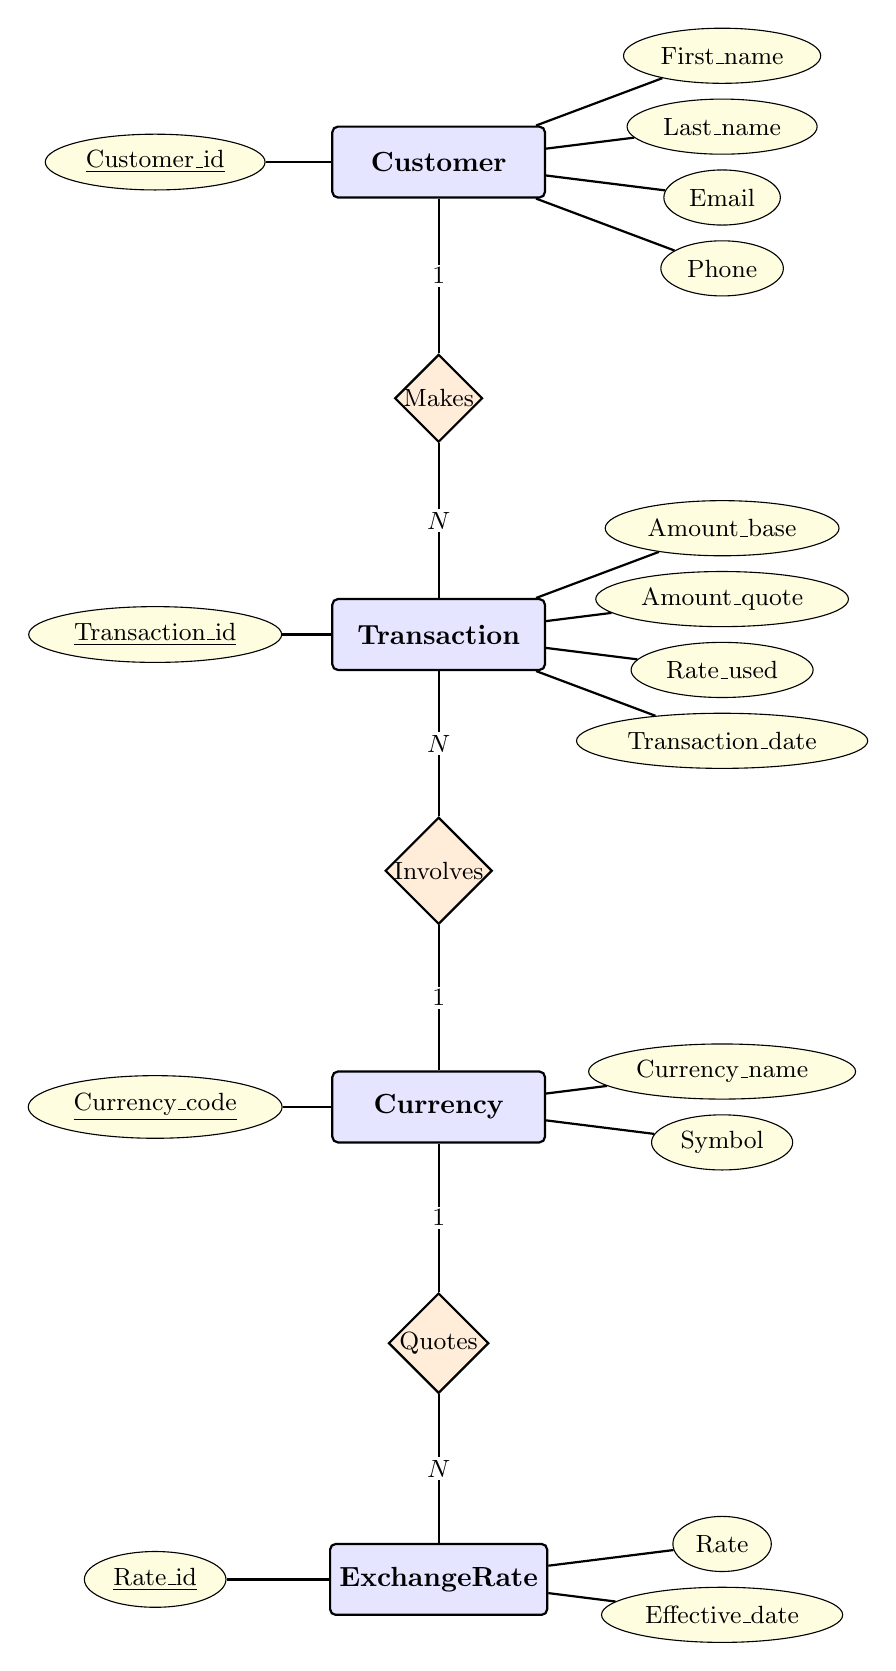
\begin{tikzpicture}[node distance=0.4cm]

    % ------------------------------------------------------------- Entities
    \node [entity] (customer)     at (0, 18) {Customer};
    \node [entity] (transaction)  at (0, 12) {Transaction};
    \node [entity] (currency)     at (0,  6) {Currency};
    \node [entity] (exchangerate) at (0,  0) {ExchangeRate};

    % -------------------------------------------------------- Relationships
    \node [rel] (makes)    at (0, 15) {Makes};
    \node [rel] (involves) at (0,  9) {Involves};
    \node [rel] (quotes)   at (0,  3) {Quotes};

    % ------------------------------------------------- Customer attributes
    \node [attrib] (cust_id)    at (-3.6, 18)    {\underline{Customer\_id}};
    \node [attrib] (first_name) at ( 3.6, 19.35) {First\_name};
    \node [attrib] (last_name)  at ( 3.6, 18.45) {Last\_name};
    \node [attrib] (email)      at ( 3.6, 17.55) {Email};
    \node [attrib] (phone)      at ( 3.6, 16.65) {Phone};

    % ---------------------------------------------- Transaction attributes
    \node [attrib] (txn_id)    at (-3.6, 12)    {\underline{Transaction\_id}};
    \node [attrib] (amt_base)  at ( 3.6, 13.35) {Amount\_base};
    \node [attrib] (amt_quote) at ( 3.6, 12.45) {Amount\_quote};
    \node [attrib] (rate_used) at ( 3.6, 11.55) {Rate\_used};
    \node [attrib] (txn_date)  at ( 3.6, 10.65) {Transaction\_date};

    % ------------------------------------------------ Currency attributes
    \node [attrib] (curr_code) at (-3.6, 6)    {\underline{Currency\_code}};
    \node [attrib] (curr_name) at ( 3.6, 6.45) {Currency\_name};
    \node [attrib] (symbol)    at ( 3.6, 5.55) {Symbol};

    % --------------------------------------------- ExchangeRate attributes
    \node [attrib] (rate_id)  at (-3.6, 0)    {\underline{Rate\_id}};
    \node [attrib] (rate)     at ( 3.6, 0.45) {Rate};
    \node [attrib] (eff_date) at ( 3.6,-0.45) {Effective\_date};

    % ----------------------------------------- Connectors (behind the shapes)
    \begin{scope}[on background layer]

      % -------- relationship connectors
      \draw [edge] (customer)     -- (makes)      node [card, pos=0.5] {$1$};
      \draw [edge] (makes)        -- (transaction) node [card, pos=0.5] {$N$};
      \draw [edge] (transaction)  -- (involves)   node [card, pos=0.5] {$N$};
      \draw [edge] (involves)     -- (currency)   node [card, pos=0.5] {$1$};
      \draw [edge] (currency)     -- (quotes)     node [card, pos=0.5] {$1$};
      \draw [edge] (quotes)       -- (exchangerate) node [card, pos=0.5] {$N$};

      % -------- customer
      \draw [edge] (customer) -- (cust_id);
      \draw [edge] (customer) -- (first_name);
      \draw [edge] (customer) -- (last_name);
      \draw [edge] (customer) -- (email);
      \draw [edge] (customer) -- (phone);

      % -------- transaction
      \draw [edge] (transaction) -- (txn_id);
      \draw [edge] (transaction) -- (amt_base);
      \draw [edge] (transaction) -- (amt_quote);
      \draw [edge] (transaction) -- (rate_used);
      \draw [edge] (transaction) -- (txn_date);

      % -------- currency
      \draw [edge] (currency) -- (curr_code);
      \draw [edge] (currency) -- (curr_name);
      \draw [edge] (currency) -- (symbol);

      % -------- exchange rate
      \draw [edge] (exchangerate) -- (rate_id);
      \draw [edge] (exchangerate) -- (rate);
      \draw [edge] (exchangerate) -- (eff_date);

    \end{scope}

  \end{tikzpicture}
  }
  \caption{ER diagram in Chen notation. Primary keys are underlined. Foreign
           keys are carried by the relationships rather than shown as
           attributes.}
\end{figure}

\noindent\textbf{Legend:} rectangles are entities, diamonds are relationships,
ellipses are attributes, and underlined attributes are primary keys.

\end{document}
